\chapter{Crescimento de Funções}

Os modelos que aprendemos a construir para avaliar o tempo de processamento de um algoritmo contém uma série de constantes que dependem do contexto em que os experimentos serão feitos -- processador, memória, sistema operacional etc.
Uma teoria para comparar algoritmos deveria abstrair esses valores e focar apenas naquilo que se mantém válido em todos os contextos.

Assim, quando comparamos a eficiência de dois algoritmos vamos comparar o tempo processamento de cada um deles como uma função do tamanho da entrada.
Além disso, vamos focar especificamente no que acontece para valores grandes da entrada.
Em outras palavras, vamoas analisar as funções de maneira {\em assintótica}.

Considere os dois modelos que vimos no capítulo anterior:

\begin{eqnarray*}
  g(n) & = & a \cdot n + b\\
  f(n) & = & c \cdot log_2(n) + d
\end{eqnarray*}

Dependendo das constantes $a$, $b$, $c$ e $d$, os valores de $f(n)$ podem ser maiores do que de $g(n)$ para certos valores de $n$.
Mas o $g$ cresce tão mais rápido que $f$ que conforme aumentamos o valor de $n$, eventualmente $g$ supera $f$ e se mantém maior para sempre independente dos valores das constantes.
Dizemos que, assintoticamente $g$ cresce mais rápido do que $f$.

De fato, nos experimentos que fizemos, é possível notar que a busca binária é mais eficiente do que a sequencial apenas quando começamos a testar com sequências grandes.

\begin{figure}
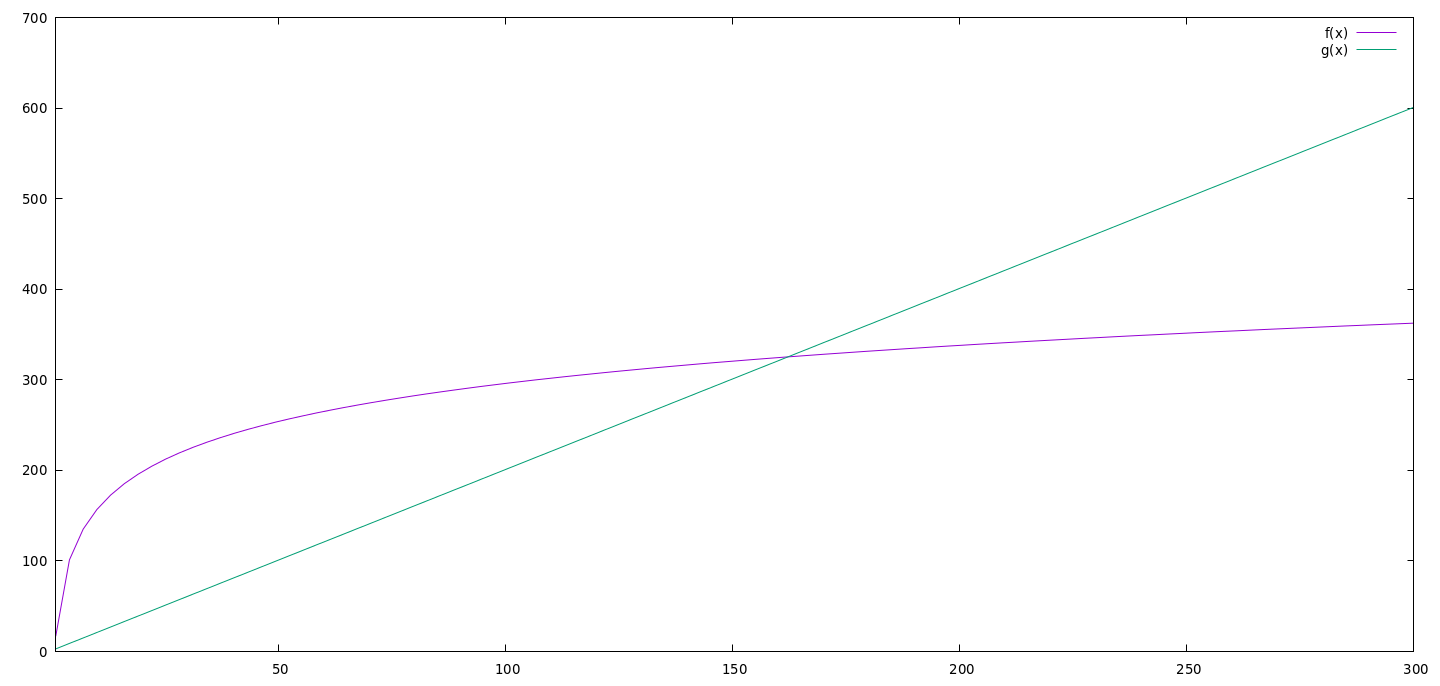
\includegraphics[width=\textwidth]{imagens/grafico7.png}
\caption{Crescimento das funções $g(n) = 2n+1$ e $f(x) = 42 \cdot log_2(n) + 17$. Há um ponto em que as curvas se cruzam e então $g(n)$ passa a ser sempre maior do que $f(n)$.}
\end{figure}

Como nos interessa analisar o comportamento assintótico das funções, trataremos como equivalentes funções que crescem de maneira similar uma vez que abstraimos as constantes.

A notação $\Theta$ formaliza matematicamente essa ideia:

\begin{displaymath}
  \Theta(g(n)) := \{ f(n) : \exists c_1, c_2, n_0 \textrm{ tal que } 0 \leq c_1 g(n) \leq f(n) \leq c_2 g(n) \forall n \geq n_0 \}
\end{displaymath}

Ou seja, $\Theta(g(n))$ é o conjunto de todas as funções que crescem de maneira parecida com $g$, que são {\em assintoticamente equivalentes} a $g$.

\begin{example}
  \begin{displaymath}
    3  n^2 + 2 n \in \Theta(n^2) 
  \end{displaymath}

  Para mostrar isso, temos que encontrar constantes $c_1$, $c_2$ e $n_0$ tais que $0 \leq c_1 n^2 \leq 3 n^2 + 2 n \leq c_2 n^2$ para todo $n \geq n_0$.

  Vamos considerar apenas valores de $n \geq 1$.
  Neste caso, $n^2$ é sempre positivo e podemos dividir tudo por $n^2$ sem alterar a direção das ineqações.
  Obtemos então:

  \begin{displaymath}
   c_1 \leq 3 + \frac{2}{n} \leq c_2
  \end{displaymath}

  Agora fica fácil ver que para $c_1 = 3$ e $c_2 = 5$ temos que as inequações valem para qualquer $n \geq 1$:

  \begin{displaymath}
   3 n^2 \leq 3 n^2 + 2n \leq 5 n^2
  \end{displaymath}

  \begin{figure}
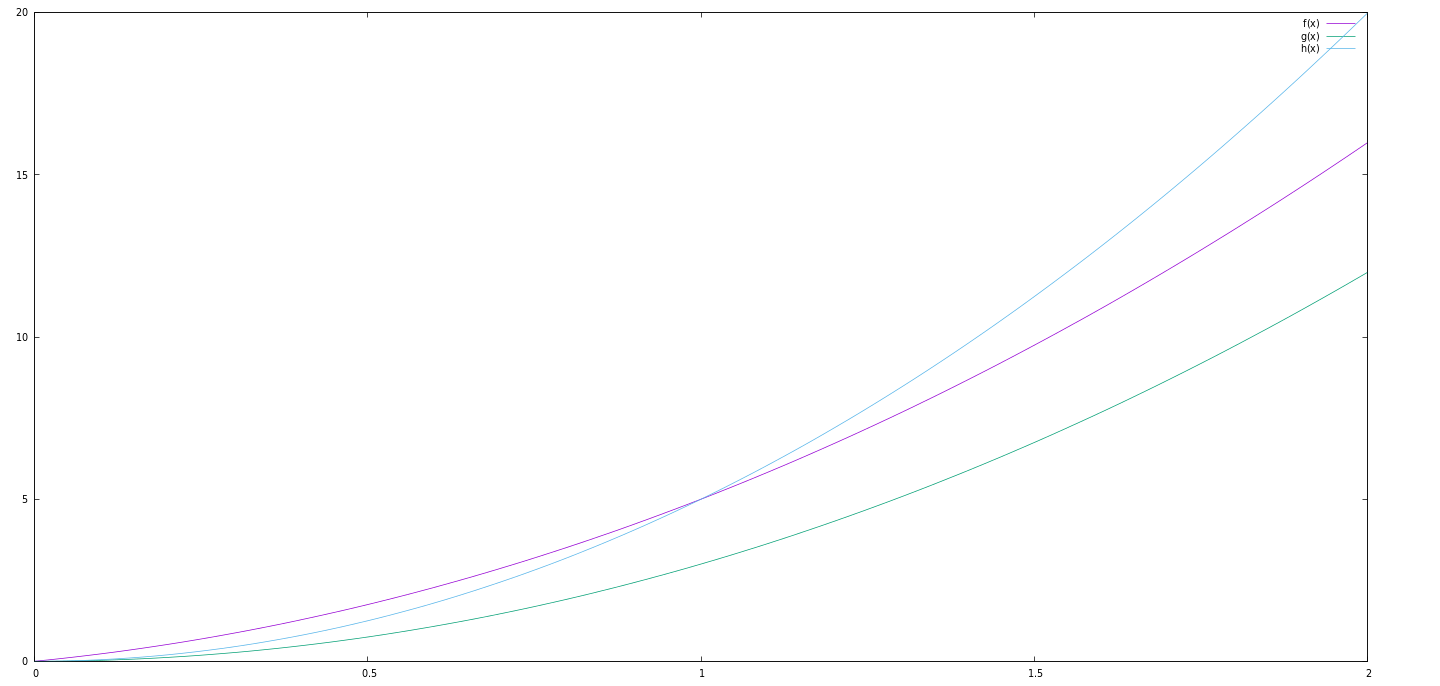
\includegraphics[width=\textwidth]{imagens/grafico5.png}
\caption{A função $f(x) = 3n^2 + 2n$ cresce de maneira assintóticamente equivalente a função $n^2$ porque $g(x) = 5n^2$ cresce mais rápido que $f$ e $h(x) = 3n^2$ cresce mais devagar que $f$.}
\end{figure}
\end{example}

\begin{example}
  \begin{displaymath}
    4  n^4 - 2 n^2 + 2 \in \Theta(n^4) 
  \end{displaymath}

   Para mostrar isso, temos que encontrar constantes $c_1$, $c_2$ e $n_0$ tais que $0 \leq c_1 n^4 \leq 4 n^4 + 2 n^2 + 2 \leq c_2 n^4$ para todo $n \geq n_0$.

   Novamente, para $n \geq 1$, $n^4$ é sempre positivo e podemos dividir tudo por $n^2$ para obter:

  \begin{displaymath}
   c_1 \leq 4 - \frac{2}{n^2} + \frac{2}{n^4} \leq c_2
  \end{displaymath}

  O valor da função $4  \frac{2}{n^2} + \frac{2}{n^4}$ é maior do que $2$ para e menor do que $6$ qualquer valor $n \geq 1$.

  Assim, temos que para todo $n \geq 1$:

  \begin{displaymath}
   2n^4 \leq 4n^4 -2n^2  + 2 \leq 6n^4
  \end{displaymath}

  \begin{figure}
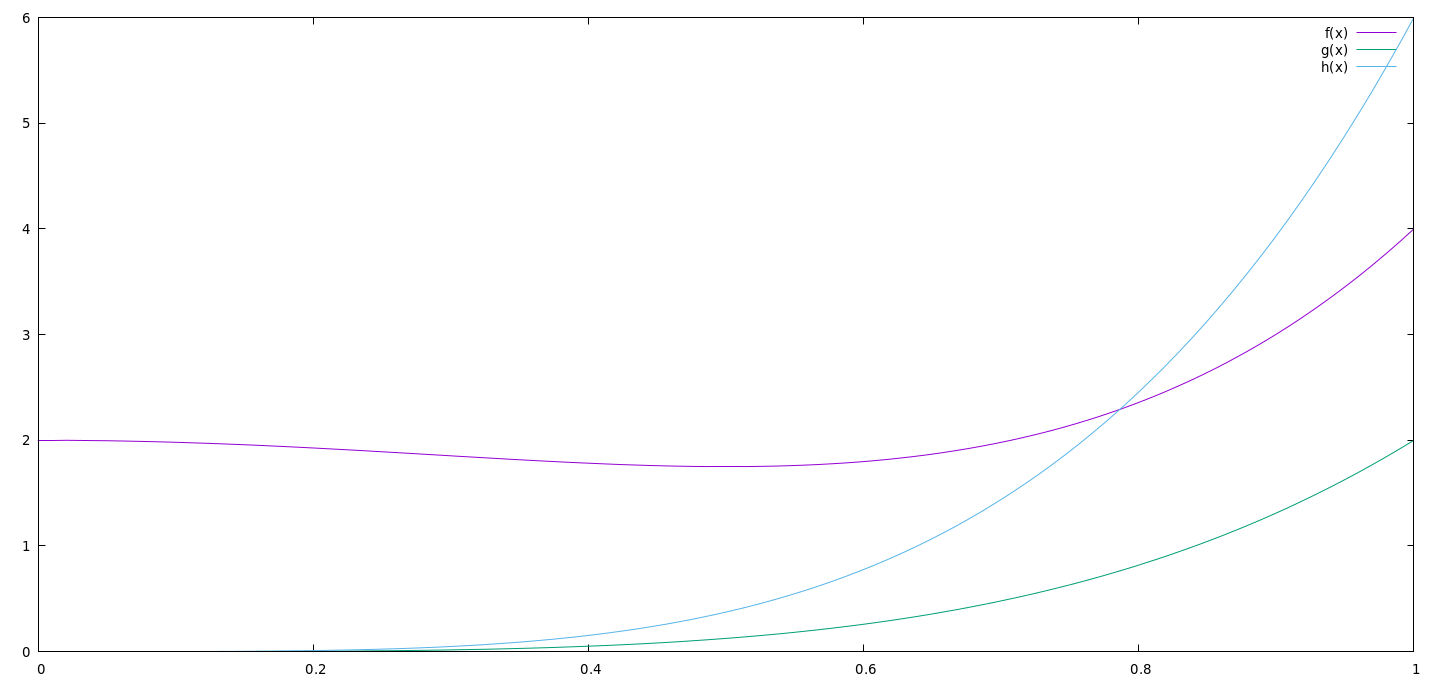
\includegraphics[width=\textwidth]{imagens/grafico6.png}
\caption{A função $f(x) = 2n^4 - 2n + 2$ cresce de maneira assintóticamente equivalente a função $n^4$ porque $g(x) = 6n^4$ cresce mais rápido que $f$ e $h(x) = 2n^4$ cresce mais devagar que $f$.}
\end{figure}

  
\end{example}

\begin{example}
  \begin{displaymath}
  2n^3 \notin \Theta(n^2)
  \end{displaymath}

  Suponha por absurdo que existam $c$, e $n_0$ tais que $2n^3 \leq c$ para todo $n \geq n_0$.

  Considerando $n > 0$ e dividindo os dois lados por $n^2$, temos:
  \begin{displaymath}
    2n \leq c
  \end{displaymath}

  Mas não é difícil ver que $2n > c$ assim que $n \geq \frac{c}{2}$, contrariando a suposição.
\end{example}

Os últimos três exemplos sugerem uma regra geral: todo polinômio é assintoticamente equivalente ao seu fator dominante.

De fato, esse resultado pode ser enunciado formalmente:

\begin{theorem}
  Seja $p(n) = a_dn^d + a_{d-1}n^{d-1} + \dots + a_0$ com $a_d > 0$ então $p(n) \in \Theta(n^d)$
\end{theorem}

\begin{corollary}
  \begin{displaymath}
    a \cdot n + b \in \Theta(n)
  \end{displaymath}
\end{corollary}

Dizemos que o consumode de tempo do algortimos Busca Sequencial é $\Theta(n)$, ou simplesmente que o algoritmo é {\em linear}.

Já o consumo de tempo do algoritmo Busca Binária, como mostra o próximo exemplo, é $\Theta(log(n))$, ou {\em logarítmico}.

\begin{example}
  \begin{displaymath}
    a \cdot log_2(n) + b \in \Theta(log(n)) 
  \end{displaymath}

   Para mostrar isso, temos que encontrar constantes $c_1$, $c_2$ e $n_0$ tais que $0 \leq c_1 log(n) \leq a \cdot log_2(n) + b \leq c_2 log(n)$ para todo $n \geq n_0$.

   Dividindo tudo por $log(n)$, temos:

   \begin{displaymath}
     c_1 \leq \frac{a}{log(2)} + \frac{b}{log(n)} \leq c_2 
   \end{displaymath}

   Fica fácil ver que as inequações valem para $c_1 = \frac{a}{log(2)}$ e $c_2 = \frac{a}{log(2)} + b$ para qualquer $n \geq 1$.   
\end{example}

Algumas classes de funções são bastante recorrentes ao analisar o tempo de processamento de algoritmos, tanto que nos referiremos a elas por um nome específico:

\begin{itemize}
\item Constante $\Theta(1)$
\item Linear $\Theta(n)$
\item Logarítmico $\Theta(log(n))$
\item Linearítmico $\Theta(n.log(n))$
\item Quadrático $\Theta(n^2)$
\item Cúbica $\Theta(n^3)$
\item Exponencial $\Theta(2^n)$
\end{itemize}

Embora a notação $\Theta$ represente um conjunto de funções, abusaremos um pouco dela para usá-la em equações.
Assim, quando escrevermos por exemplo $n\Theta(n) = \Theta(n^2)$ o que queremos dizer é que para qualquer $f(n) \in \Theta(n)$ temos que $n.f(n) \in \Theta(n^2)$.
De fato, podemos mostrar isso:

\begin{example}
  \begin{displaymath}
    n\Theta(n) = \Theta(n^2)
  \end{displaymath}

  Se $f(n) \in \Theta(n)$ então, por definição, existem $c_1$, $c_2$ e $n_0$ tais que:
  \begin{displaymath}
    0 \leq c_1 \cdot n \leq f(n) \leq c_2 \cdot n \textrm{ para todo } n \geq n_0
  \end{displaymath}
  Considerando $n_0 > 0$ e multiplicando tudo por $n$ temos que:
    \begin{displaymath}
    0 \leq c_1 \cdot n^2 \leq n \cdot f(n) \leq c_2 \cdot n^2 \textrm{ para todo } n \geq n_0
  \end{displaymath}
\end{example}

Considere mais uma vez o algoritmo da Busca Sequencial.
As duas primeiras linhas são executadas $\Theta(n)$ vezes no pior caso.
Já as duas últimas $\Theta(1)$ vezes.

Como isso temos que o tempo de execução em função do tamanho da entrada $n$ no pior caso segue a seguinte função:

\begin{displaymath}
  T(n) = \Theta(n) + \Theta(n) + \Theta(1) = \Theta(n)
\end{displaymath}

\begin{example}

  Primeiro note que $\Theta(1)$ é uma constante.
  Isso porque, por definição temos que:

  \begin{displaymath}
    0 \leq c_1 \leq f_3(n) \leq c_2 \textrm{ para todo } n \geq n_1
  \end{displaymath}

  As outras duas funções precisam respeitar as seguintes inequações:

  \begin{displaymath}
    0 \leq c_3\cdot n \leq f_1(n) \leq c_4 \cdot n\textrm{ para todo } n \geq n_2
  \end{displaymath}

  \begin{displaymath}
    0 \leq c_5 \cdot n \leq f_2(n) \leq c_6 \cdot n\textrm{ para todo } n \geq n_3
  \end{displaymath}

  Somando $f_1$ e $f_2$ temos que:

  \begin{displaymath}
    0 \leq (c_3 + c_5)n \leq f_1(n) + f_2(n) \leq (c_4 + c_6)n\ \forall n \geq max(n_1,n_2)
  \end{displaymath}
  
  Se somarmos $f_3$, certamente não alteramos as inequações do lado esquerdo e do lado direito temos:

  \begin{displaymath}
    f_1(n) + f_2(n) + f_3(n)\leq (c_2 + c_4 + c_6)n\ \forall n \geq max(n_1,n_2,n_3,1)
  \end{displaymath}
  
\end{example}

  A notação $\Theta$ indica limites inferior e superior para o crescimento de uma função.
  Quando avaliamos o tempo e processamento de um algoritmo, é comum desejarmos garantir que ele seja suficientemente eficiente.
  Ou seja, em geral queremos estabelecer apenas o {\em limite assintótico superior}.
  Para tanto, utilizamos a notação $O$.

  \begin{displaymath}
    O(g(n) := \{f(n) : \exists c, n_o \textrm{ tais que } 0 \leq f(n) \leq cg(n)\ \forall n \geq n_0 \}
  \end{displaymath}

  Sempre que $f(n) \in \Theta(g(n))$ temos que $f(n) \in O(g(n))$.
  Ou seja, $\Theta(g(n)) \subseteq O(g(n))$.
  Já a recíproca não é necessariamente verdadeira:

  \begin{example}
    $n \notin \Theta(n^2)$, mas $n \in O(n^2)$

    A primeira parte é totalmente análoga ao Exemplo \ref{}.
    Para mostrar a segunda, note que:

    \begin{displaymath}
     0 \leq n \leq n^2 \textrm{ para todo } n \geq 1
    \end{displaymath}
  \end{example}

  Da mesma forma, existem situações em que nos interessa apenas o {\em limite assintótico inferior} de uma função.
  Por exemplo, quando avaliamos certos problemas computacionais, em alguns casos específicos sabemos que é impossível resolver o problema de maneira assintoticamente mais eficiente do que certa função $f(n)$.
  Nesses casos, dizemos que o problema é $\Omega(f(n))$.

  \begin{displaymath}
    \Omega(g(n) := \{f(n) : \exists c, n_o \textrm{ tais que } 0 \leq cg(n) \leq f(n)\ \forall n \geq n_0 \}
  \end{displaymath}

  Quando temos uma solução $O(g(n))$ para um problema $\Omega(g(n))$ dizemos que essa solução é {\em ótima}. 

  \begin{example}
    O problema da busca em uma sequência arbitrária é $\Omega(n)$.
    Isso porque precisamos consultar todos $n$ elementos da sequência para saber se o elemento pertence a ela ou não.

    Assim, o algoritmo de BuscaSequencial que temos estudado é ótimo para o problema da busca em sequência arbitrária, mas ele não é ótimo para o problema da busca em sequência ordenada.
    Para este segundo problema conhecemos uma solução $O(log(n))$.
  \end{example}

  \begin{theorem}
    Para qualquer função $g(n)$ temos que $f(n) \in \Theta(g(n))$ se e somente se $f(n) \in O(g(n))$ e $f(n) \in \Omega(g(n))$. Em outras palavras: $\Theta(g(n)) = O(g(n)) \cap \Omega(g(n))$
  \end{theorem}

  Quando analisamos o tempo de processamento de um algoritmo como uma função do tamanho da entrada, é consensual a simplificação de desprezar os termos não dominantes e, com isso, simplificar as contas considerando apenas o comportamento assintótico.
  Há uma controvérsia, porém, sobre a constante multiplicadora do fator dominante.
  Alguns autores a desprezam por se tratar de um valor que depende do contexto.
  Outros autores, avaliam que esse valor não deve ser desprezado.
  No primeiro caso, utilizamos a notação $\Theta$ já apresentada.
  No segundo caso, utilizamos a notação til ($\sim$).

  Assim, por exemplo, temos que:

  \begin{displaymath}
    4n^3 + 2n + 8 \sim 4n^3 \in \Theta(n^3)
  \end{displaymath}

  Já um exemplo negativo seria:

  \begin{displaymath}
    4n^3 + 2n + 8 \nsim 2n^3 
  \end{displaymath}

  Formalmente, dizemos que $f(n) \sim g(n)$ se e somente se $lim_{n \to \infty}\frac{f(n)}{g(n)} = 1$.
  
  
\begin{exercicio}
  Mostre que o tempo de processamento do algorítimo $3Soma$ é $\Theta(n^3)$ no pior caso.
\end{exercicio}
